\documentclass[mat1,reqno]{fmfdelo}
% \documentclass[fin1]{fmfdelo}
% \documentclass[isrm1]{fmfdelo}
% \documentclass[mat2]{fmfdelo}
% \documentclass[fin2]{fmfdelo}
% \documentclass[isrm2]{fmfdelo}

% aktivirajte pakete, ki jih potrebujete
% \usepackage{tikz}
\usepackage{amsmath}
\usepackage{mathtools}

\usepackage[normalem]{ulem}
\usepackage{soul}
\usepackage{cancel}
\usepackage{amssymb}
\usepackage{graphicx}
\usepackage[utf8]{inputenc}

% za številske množice uporabite naslednje simbole
\newcommand{\R}{\mathbb R}
\newcommand{\N}{\mathbb N}
\newcommand{\Z}{\mathbb Z}
\newcommand{\C}{\mathbb C}
\newcommand{\Q}{\mathbb Q}

% matematične operatorje deklarirajte kot take, da jih bo Latex pravilno stavil
% \DeclareMathOperator{\conv}{conv}

% na razpolago so naslednja matematična okolja, ki jih kličemo s parom 
% \begin{imeokolja}[morebitni komentar v oklepaju] ... \end{imeokolja}
%
% definicija, opomba, primer, zgled, lema, trditev, izrek, posledica, dokaz
% 


% vstavite svoje definicije ...
%  \newcommand{}{}


% naslednje ukaze ustrezno napolnite
\avtor{Martin Dolenc} 

\naslov{Projekt pri predmetu Matematično modeliranje}

% navedite ime mentorja s polnim nazivom: doc.~dr.~Ime Priimek, 
% izr.~prof.~dr.~Ime Priimek, prof.~dr.~Ime Priimek
% uporabite le tisti ukaz/ukaze, ki je/so za vas ustrezni 
%\mentor{}
% \mentorica{}
% \somentor{}
% \somentorica{}
% \mentorja{}{}
% \mentorici{}{}

\letnica{2021} % leto seminarja

%  V povzetku na kratko opišite vsebinske rezultate dela. Sem ne sodi razlaga organizacije dela --
%  v katerem poglavju/razdelku je kaj, pač pa le opis vsebine.
\povzetek{}

%  Prevod slovenskega povzetka v angleščino. 
\abstract{}

% navedite vsaj eno klasifikacijsko oznako --
% dostopne so na www.ams.org/mathscinet/msc/msc2010.html
\klasifikacija{}
\kljucnebesede{} % navedite nekaj ključnih pojmov, ki nastopajo v delu
\keywords{} % angleški prevod ključnih besed
\overfullrule=0pt

\begin{document}

%------------------------------------------------------------------------------------------------------------------------------------------

\newpage
\section{Uvodni problem}

Otrok se sprehaja po ravnem igrišču na mivki, za seboj pa vleče na vrvico
privezano igračo tako, da je vrvica vseskozi napeta. Denimo, da otrokovo
gibanje opišemo s parametrično ravninsko krivuljo. Napišite program, ki
izračuna sled gibanja igrače po mivki. Izriše naj tudi gibanje otroka in
igrače.

%------------------------------------------------------------------------------------------------------------------------------------------

\section{Pristop}

Problem si lahko predstavljamo kot da imamo neko točko, ki se premika po krivulji, za seboj pa vleče neko drugo točko (glej spodnjo skico).

\begin{figure}[!h]
\centering
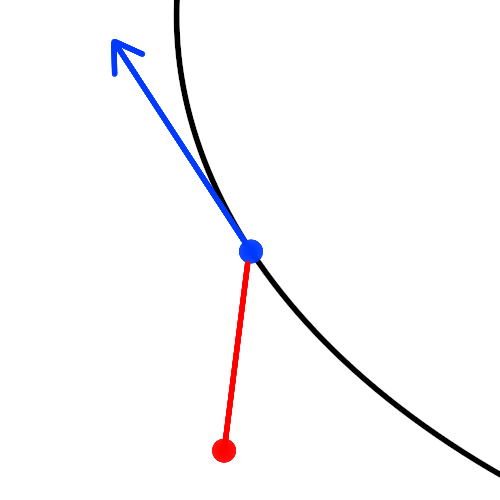
\includegraphics[scale=1]{Skica problema}\\
Skica problema.
\end{figure}

\subsection{Teoretična rešitev}

Podano imamo parametrizirano ravninsko krivuljo (zgoraj označeno z črno), ki predstavlja premikanje otroka. Iz tega da je vrvica vseskozi napeta sledi, da je razdalja med otrokom in igračo konstantna (označeno z rdečo črto) in da se igrača vedno giblje v smeri proti otroku. Zdaj lahko izrazimo hitrost igrače s pomočjo hitrosti otroka (označena z modro puščico) in kota med smerjo gibanja igrače in smerjo gibanja otroka. Tako dobimo diferencialno enačbo prvega reda katere rešitev bo opisovala pot igrače na igrišču.

Za reševanje same diferencialne enačbe bomo izkoristili Matlabovo funkcijo {\texttt{ode45}}, ki nam bo vrnila pot igrače.

%------------------------------------------------------------------------------------------------------------------------------------------

\section{Reševanje uvodnega problema}

Z $x_{o}(t)$ in $y_{o}(t)$ označimo parametrizacijo krivulje po kateri se sprehaja otrok, z $x_{i}(t)$ in $y_{i}(t)$ pa pot igrače. Vemo da vektor hitrosti igrače vedno kaže proti otroku, to lahko zapišemo kot

$$x_{i}'(t) = a \cdot (x_{o}(t) - x_{i}(t)),$$
$$y_{i}'(t) = a \cdot (y_{o}(t) - y_{i}(t)),$$

za nek $a \in \mathbb R$.

Vpeljimo še oznaki

\begin{equation*}
x_{r}(t) = x_{o}(t) - x_{i}(t) \quad \textrm{in} \quad
y_{r}(t) = y_{o}(t) - y_{i}(t)
\end{equation*}

za lažji zapis.

Vektor smeri igrače normiramo, ga pomnožimo z normo hitrosti otroka in to označimo z $v(t)$.

\begin{equation}\label{enačba:v}
v(t) = \frac{
\begin{bmatrix}
	x_{r}(t) \\
	y_{r}(t)
\end{bmatrix}
}
{
\begin{Vmatrix}
\begin{bmatrix}
	x_{r}(t) \\
	y_{r}(t)
\end{bmatrix}
\end{Vmatrix}
}
\cdot
\begin{Vmatrix}
\begin{bmatrix}
	x_{o}'(t) \\
	y_{o}'(t)
\end{bmatrix}
\end{Vmatrix}
\end{equation}
\\

Seveda $v(t)$ še ni končni rezultat, zgornja enačba velja samo v primeru ko se otrok giblje po premici in mu igrača sledi za petami. Če želimo enačbo ki bo veljala za vse primere, moramo upoštevati še kot med smerjo gibanja igrače in smerjo gibanja otroka, zato pa bomo uporabili formulo za kosinus kota med tema dvema vektorjema.

\begin{equation}\label{enačba:cos}
\cos(\alpha(t)) = \frac{
\begin{bmatrix}
	x_{o}'(t) & y_{o}'(t)
\end{bmatrix}
\cdot
\begin{bmatrix}
	x_{r}(t) \\
	y_{r}(t)
\end{bmatrix}
}{
\begin{Vmatrix}
\begin{bmatrix}
	x_{o}'(t) \\
	y_{o}'(t)
\end{bmatrix}
\end{Vmatrix}
\cdot
\begin{Vmatrix}
\begin{bmatrix}
	x_{r}(t) \\
	y_{r}(t)
\end{bmatrix}
\end{Vmatrix}
}
\end{equation}
\\
kjer je $\alpha(t)$ kot med vektorjema, ki predstavljata smeri gibanj otroka in igrače. Zdaj lahko z $v(t)$ in $\alpha(t)$ zapišemo hitrost igrače

\begin{equation*}
\begin{bmatrix}
	x_{i}'(t) \\
	y_{i}'(t)
\end{bmatrix} = \cos(\alpha(t)) \cdot v(t)
\end{equation*}

in zdaj namesto $\cos(\alpha(t))$ in $v(t)$ vstavimo to kar smo zapisali pri (\ref{enačba:v}) in (\ref{enačba:cos}) in dobimo

\begin{equation*}
\begin{bmatrix}
	x_{i}'(t) \\
	y_{i}'(t)
\end{bmatrix} = \frac{
\begin{bmatrix}
	x_{r}(t) \\
	y_{r}(t)
\end{bmatrix}
\cdot
\Big(
\begin{bmatrix}
	x_{o}'(t) & y_{o}'(t)
\end{bmatrix}
\cdot
\begin{bmatrix}
	x_{r}(t) \\
	y_{r}(t)
\end{bmatrix}
\Big)
}{
\begin{Vmatrix}
\begin{bmatrix}
	x_{r}(t) \\
	y_{r}(t)
\end{bmatrix}
\end{Vmatrix}^2
}.
\end{equation*}
\\

Če zdaj v enačbi zamenjamo $x_{r}(t)$ in $y_{r}(t)$, dobimo

\begin{equation*}
\begin{bmatrix}
	x_{i}'(t) \\
	y_{i}'(t)
\end{bmatrix} = \frac{
\begin{bmatrix}
	x_{o}(t) - x_{i}(t)) \\
	y_{o}(t) - y_{i}(t)
\end{bmatrix}
\cdot
\Big(
\begin{bmatrix}
	x_{o}'(t) & y_{o}'(t)
\end{bmatrix}
\cdot
\begin{bmatrix}
	x_{o}(t) - x_{i}(t) \\
	y_{o}(t) - y_{i}(t)
\end{bmatrix}
\Big)
}{
\begin{Vmatrix}
\begin{bmatrix}
	x_{o}(t) - x_{i}(t) \\
	y_{o}(t) - y_{i}(t)
\end{bmatrix}
\end{Vmatrix}^2
}.
\end{equation*}
\\

Kar je diferencialna enačba za $x_{i}(t)$ in $y_{i}(t)$. Začetni problem je pa določen z $x_{i}(0) = x_{0}$ in $y_{i}(0) = y_{0}$, kjer sta $x_{0}$ in $y_{0}$ začetni koordinati igrače.

%------------------------------------------------------------------------------------------------------------------------------------------

\section{Opis priloženih datotek}

V datoteki {\texttt{Main.m}} se izvaja glavni program, tukaj lahko določimo začetne parametre in potem z zagonom scripte vidimo potovanje otroka in igrače. V programu kličemo funkciji {\texttt{narisi\_pot\_otroka.m}} in {\texttt{narisi\_pot\_igrace.m}}, ki izrišesta poti otroka in igrače, s funkcijo {\texttt{animacija.m}} pa animiramo premikanje le teh. Večino računanja pa poteka v funkciji {\texttt{resi\_enacbo\_za\_igraco.m}} kjer rešimo diferencialno enačbo, ki smo jo zapisali v prejšnjem poglavju.

%------------------------------------------------------------------------------------------------------------------------------------------

\newpage

\section{Primeri gibanj otroka in igrače}

Spodaj je prikazanih nekaj primerov gibanja otroka in igrače. Z modro je označena krivulja po kateri se sprehaja otrok, z rdečo pa sled, ki jo pusti za seboj igrača.

%---------------------------

\subsection{Delna elipsa} Pri temu primeru smo za krivuljo vzeli:

\begin{equation*}
x_{o}(t) = 3\cos(t) \quad \textrm{in} \quad
y_{o}(t) = 2\sin(t)
\end{equation*}
\\
Začetni čas je $\frac{\pi}{2}$, končni pa $2\pi$. Začetne koordinate igrače pa so $x_{0} = 0$ in $y_{0} = 0$.

\begin{figure}[!h]
\centering
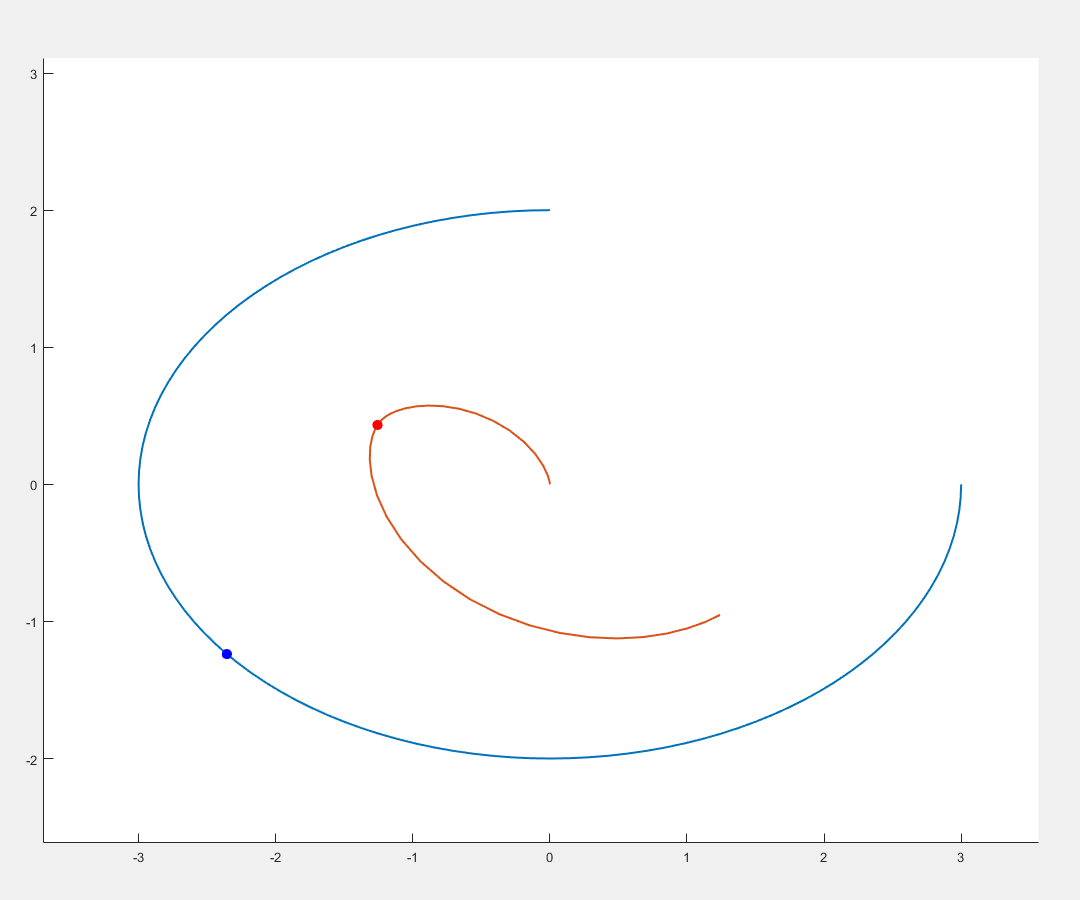
\includegraphics[scale=0.2]{Delna elipsa}\\
Delna elipsa.
\end{figure}

%---------------------------

\subsection{Spirala} Pri temu primeru smo za krivuljo vzeli:

\begin{equation*}
x_{o}(t) = t\cos(t) + 1 \quad \textrm{in} \quad
y_{o}(t) = t\sin(t)
\end{equation*}
\\
Začetni čas je $0$, končni pa $2\pi$. Začetne koordinate igrače pa so $x_{0} = 0$ in $y_{0} = 0$.

\begin{figure}[!h]
\centering
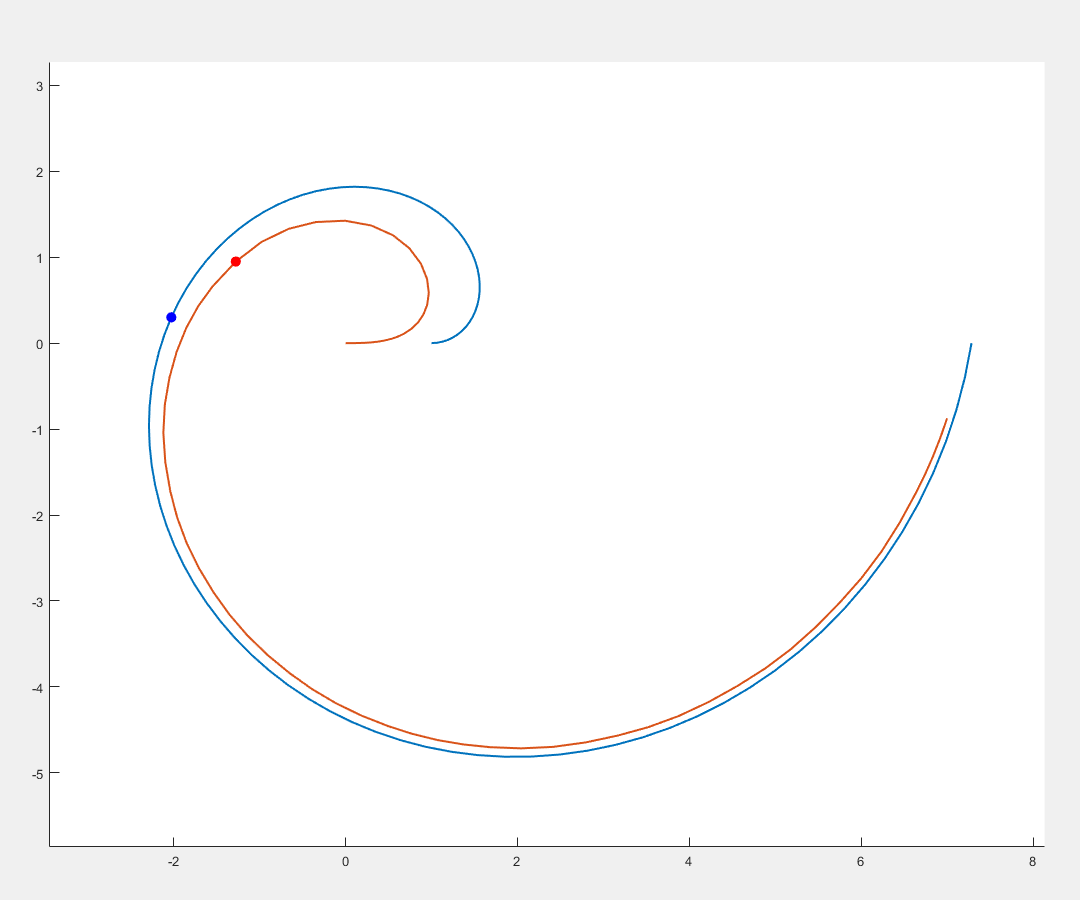
\includegraphics[scale=0.2]{Spirala}\\
Spirala.
\end{figure}

%---------------------------

\subsection{Elipsa z zamaknjenim začetkom} Pri temu primeru smo za krivuljo vzeli:

\begin{equation*}
x_{o}(t) = 2\cos(t) \quad \textrm{in} \quad
y_{o}(t) = 3\sin(t)
\end{equation*}
\\
Začetni čas je $0$, končni pa $2\pi$. Začetne koordinate igrače pa so $x_{0} = 2$ in $y_{0} = -2$.

\begin{figure}[!h]
\centering
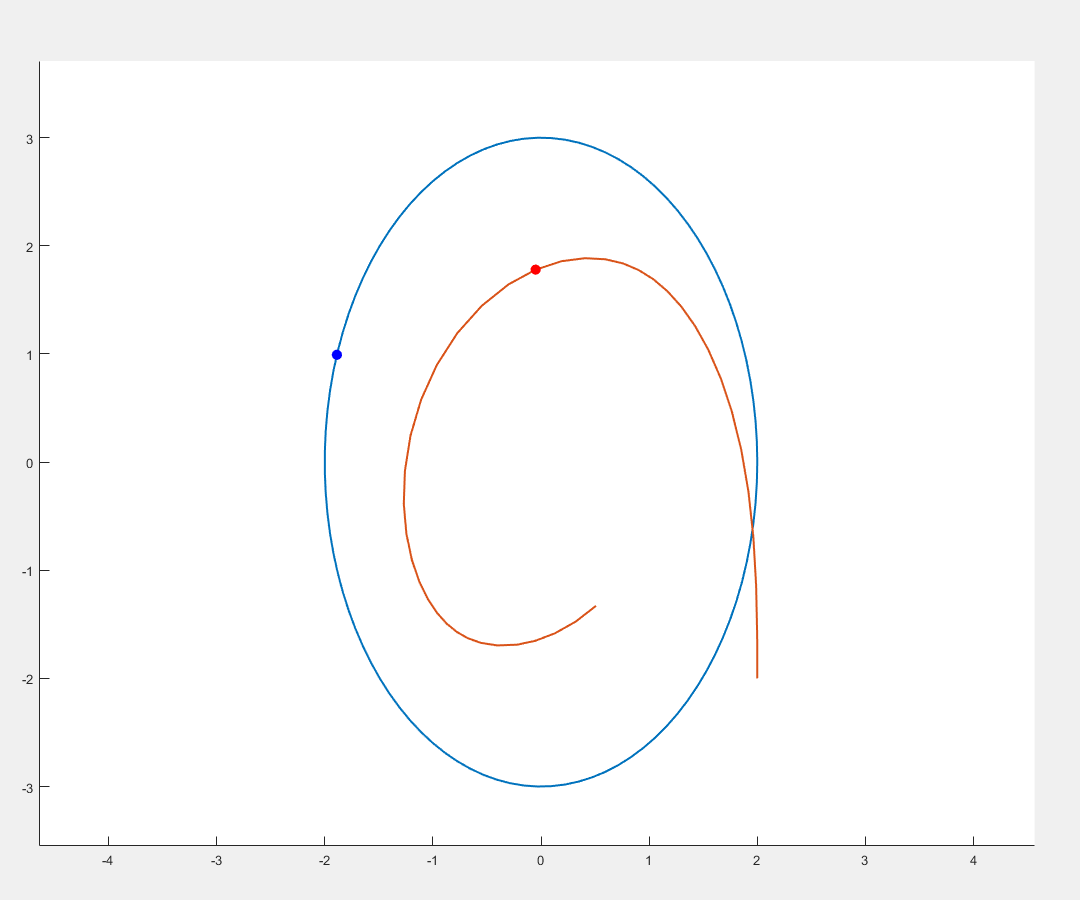
\includegraphics[scale=0.2]{Elipsa z zamaknjenim začetkom}\\
Elipsa z zamaknjenim začetkom.
\end{figure}


%------------------------------------------------------------------------------------------------------------------------------------------

\newpage

% seznam uporabljene literature
\begin{thebibliography}{99}

\bibitem{referenca-spletni-vir}
F.~Forstnerič, \emph{Navadne diferencialne enačbe in variacijski račun}, verzija 5.~9.~2021, [ogled 5.~9.~2021], dostopno na \url{https://ucilnica.fmf.uni-lj.si/pluginfile.php/94347/mod_resource/content/0/Skripta.pdf}.

\end{thebibliography}

\end{document}

